\section{Der Optimierungsvorgang}

\begin{figure}[h]
  \centering
  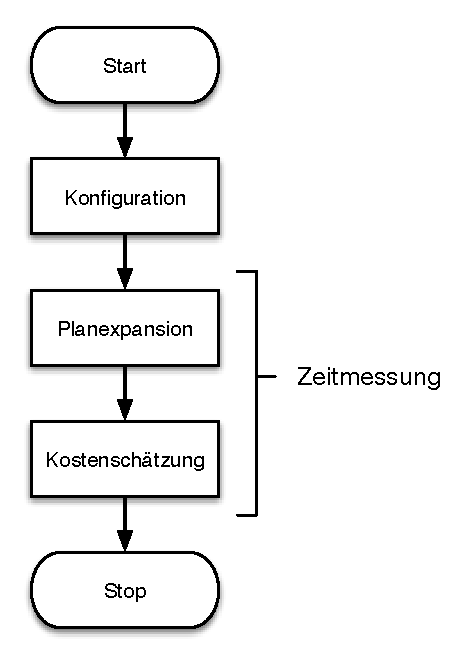
\includegraphics{04_Implementierung/00_media/Ablauf.pdf}
  \caption{Ablauf der eigenen Implementierung}
  \label{Ablauf}
\end{figure}

Die Ausführung des Programms geschieht in drei Schritten (vgl. Abb. \ref{Ablauf}): (1) Konfiguration, (2) Generierung von semantisch gleichen Plänen, (3) Finden des optimalen Plans.




Im ersten Schritt, wird auf Grund von externen Parametern das System konfiguriert. Die Konfiguration erfolgt durch ein JSON File. In ihm werden die Parameter (Relationen und deren Kardinalität, Join-Kanten und deren Selektivität, initaler Plan und Regelsets) für die Optimierung festgelegt. Mit Hilfe der Relationen und deren Kardinalität können später im Zusammenspiel mit Join-Kanten und Selektivitität die Kosten für einen Plan berechnet werden. Der initiale Plan dient als Startpunkt der Transformation. Auf ihn werden die Regelmengen angewendet und so logische  Äquivalente erzeugt.

Zu Beginn des zweiten Schritts, der Erzeugung von äquivalenten Plänen, wird die Zeitmessung gestartet.  Mit Hilfe von Enumeratoren werden die unterschiedlichen Regelmengen auf den initialen Plan angewendet.

In einem finalen Schritt findet die Kostenberechnung statt um aus den möglichen Plänen den günstigsten auszuwählen. Diese Preisberechnung wird im Modul der Kostenschätzung vollzogen.



\begin{figure}[ht]
  \centering
  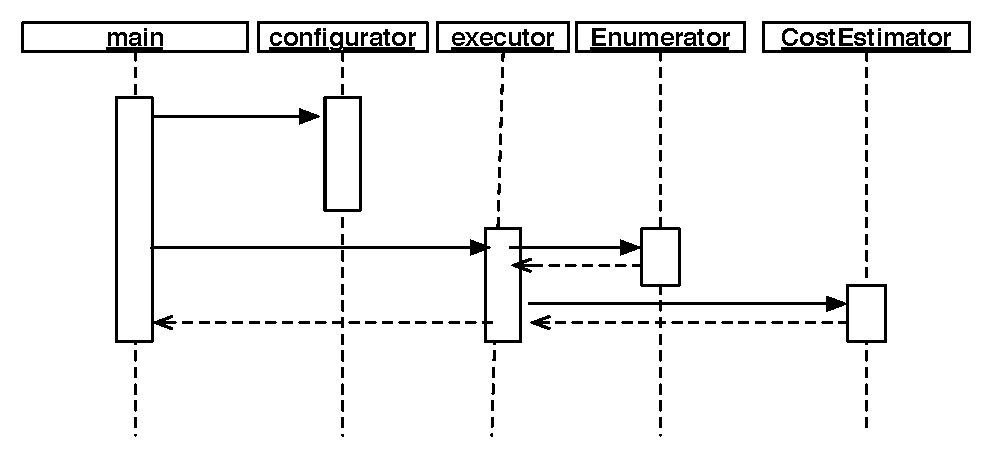
\includegraphics[width=\textwidth]{04_Implementierung/00_media/SequenceDiagramConfiguration.pdf}
  \caption{Sequenzdiagramm: Aufruf der einzelnen Komponenten}
  \label{SequenceDiagramConfiguration}
\end{figure}


Die genaue Reihenfolge der Aufrufe beginnend mit der Hauptmethode lässt sich in Abbildung \ref{SequenceDiagramConfiguration}, einem Sequenzdiagramm, am besten ablesen. Zuerst muss die Konfiguration abgefragt werden. Diese Konfiguration wird dann an einen Exektor weitergegeben, der für Zusammenstellung von Regelmengen und Enumerator verantworlich ist, ebenfalls ruft er die Kostenschätzung auf und ruft die Zeitmessung auf. Die einzelnen Komponenten werden im Folgenden genau besprochen.
